\section{Data Structure}
\label{sec:data_structure}
The data for this task is provided in two files: \textit{test.csv} and \textit{train.csv}. The training set contains approximately 20,000 labelled sentences, and the test set contains approximately 8,000 unlabelled sentences.

The data is provided in the form described in Table \ref{tab:data_form}.

\begin{table}[h]
\centering
\begin{tabular}{|c|c|c|}
\hline 
\textbf{id} & \textbf{text} & \textbf{author} \\ 
\hline 
id26305 & This process, however, \ldots & EAP \\ 
\hline 
id17569 & It never once occurred \ldots & HPL \\ 
\hline 
\ldots & \ldots & \ldots \\ 
\hline 
\end{tabular} 
\caption{The provided data, as in \textit{test.csv}.}
\label{tab:data_form}
\end{table}
The three authors represented in this dataset are Edgar Allen Poe (\textit{EAP}), H.P Lovecraft (\textit{HPL}), and Mary Shelley (\textit{MWS}.

\subsection{Balanced Data}
\label{sec:balanced_data}

There is a slight bias in the dataset, but it is approximately balanced as shown in Figure \ref{fig:balance}. This should allow model training to work well without balancing of the training data.

\begin{figure}[h]
\centering
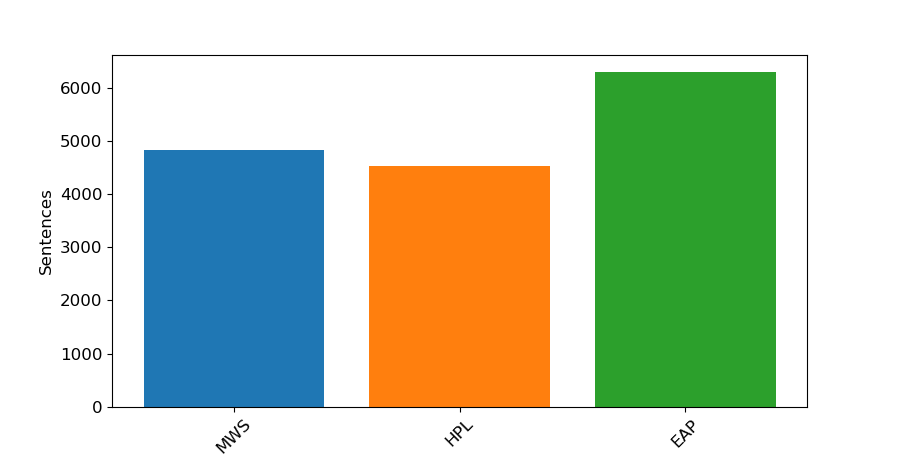
\includegraphics[width=\columnwidth]{Figures/Data_Structure/balance.png}
\caption{Number of sentences in the training set, by author}
\label{fig:balance}
\end{figure}

\subsection{Sentence Lengths}
\label{sec:sentence_lengths}

A broad examination of the data offers some insight into the difference between these authors' styles. The first and most obvious attribute to examine is the sentence length, which is shown in Figure \ref{fig:senlen}. Whilst the three authors are all largely similar in their distribution of sentence lengths, there is a noticeable difference. This may, therefore, provide a useful feature for discriminating between classes.

\begin{figure}[h]
\centering
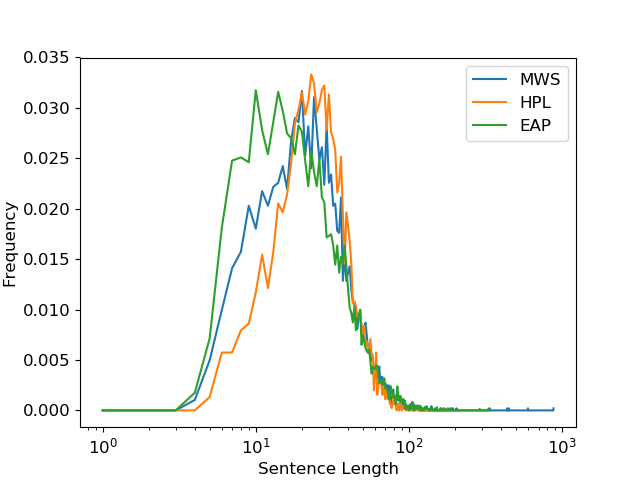
\includegraphics[width=\columnwidth]{Figures/Data_Structure/senlen.png}
\begin{tabular}{|c|c|c|}
\hline  
\textbf{Author} & \textbf{Mean} & \textbf{Standard Deviation} \\ 
\hline 
MWS & 31.3 & 26.0 \\ 
\hline 
HPL & 30.8 & 15.3 \\ 
\hline 
EAP & 29.4 & 21.1 \\ 
\hline 

\end{tabular} 
\caption{Sentence length frequency, by author}
\label{fig:senlen}
\end{figure}

\subsection{Word Frequency}
\label{sec:word_frequency}

Another obvious way in which the authors may differ is their word choice; They are likely to favour different words, and their occurrence in a sentence may evidence their author.

Figure \ref{fig:wordfreq_before} shows the most frequent words used by each author, and is not particularly useful; The majority of them are shared between authors. Removing stopwords produces the results in Figure \ref{fig:wordfreq_after}, which more uniquely identify the authors. At a glance these word sets don't seem to overlap a great deal, and so classifying sentences by the likelihood of each author to write it may be a productive approach.

\begin{figure}[h]
\centering
\begin{subfigure}[b]{\columnwidth}
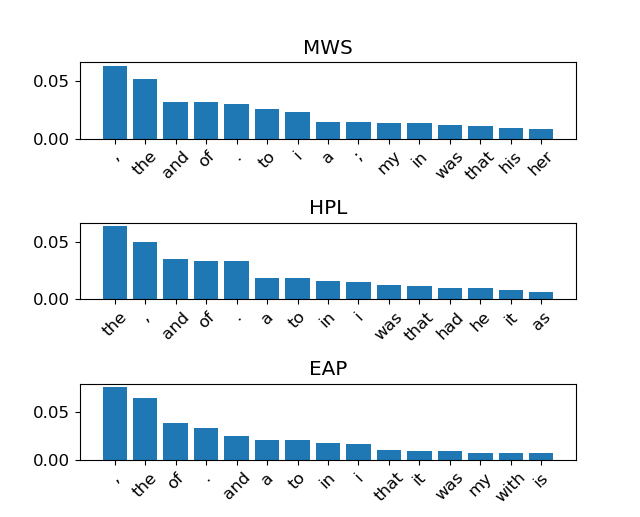
\includegraphics[width=\textwidth]{Figures/Data_Structure/wordfreq_before.png}
\caption{20 most used words, by author, before stopword removal}
\label{fig:wordfreq_before}
\end{subfigure} \\
\begin{subfigure}[b]{\columnwidth}
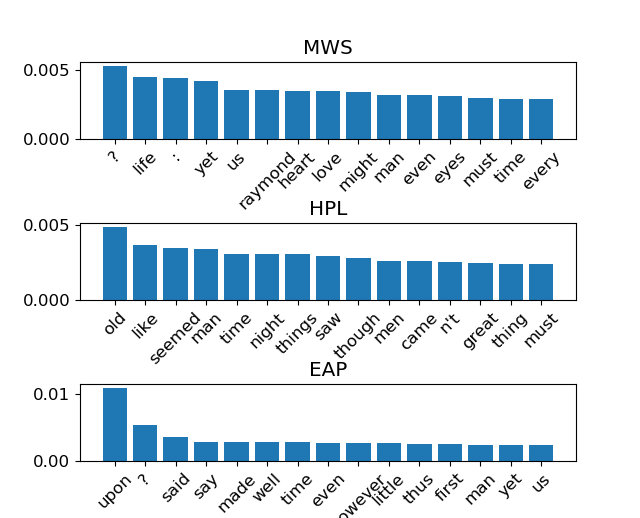
\includegraphics[width=\textwidth]{Figures/Data_Structure/wordfreq_after.png}
\caption{20 most used words, by author, after stopword removal}
\label{fig:wordfreq_after}
\end{subfigure}
\caption{Author word usage}
\label{fig:wordfreq}
\end{figure}

